\documentclass[11pt, a4paper, abstract=true]{scrartcl}
\usepackage[sexy]{evan}
\usepackage{float}
\usepackage[margin=1.00in]{geometry}
\usepackage{multirow}
\usepackage{longtable}
\usepackage{chemformula}
\def\arraystretch{1.20}
%\clearpairofpagestyles
\setkomafont{pagenumber}{\itshape}
\KOMAoptions{}
\ohead{\footnotesize \textbf{\leftmark}}
\ihead{\footnotesize \textsc{Lab Report IV}}
\cfoot{\pagemark}
\begin{document}
\subject{CH1202: Lab Report IV}
\title{
\huge Determination of the Strength of a Solution of a Strong Acid through Conductometric Titration
}
\author{
Abhisruta Maity \\
{\normalsize 21MS006}
\plusemail{am21ms006@iiserkol.ac.in}
}
\date{}
\publishers{
\normalsize \emph{Indian Institute of Science Education and Research, Kolkata \\
Mohanpur, West Bengal, 741246, India}
}
\maketitle
\tableofcontents

\section{Brief Theory and Equation}

For a solution containing electrolytes, the conductance is defined as: \[G = \frac{1}{R} = \frac{1}{\rho \frac{l}{A}} = \kappa \frac{A}{l}\] where \(\kappa\) is the conductivity (in other words, specific conductance) of the solution.

In aqueous solution of HCl, if we gradually add the NaOH, the following reaction will take place: \[\ch{H+ + Cl- + Na+ + OH- <=> Na+ + Cl- + H2O}\] We observe, if we add NaOH then the conductivity decreases since \ch{H+} is used up to react with \ch{OH-} and replaced by \ch{Na+} and \ch{OH-} which have relatively low conductivities. This happens till the equivalence point. Then, adding more NaOH increases \ch{OH-} in the solution, consequently increasing the conductivity.
\section{Dataset}

\begin{itemize}
    \item Weight of Oxalic Acid taken = 1.2607 g
\end{itemize}

\begin{table}[H]
    \centering
    \begin{tabular}{|c|c|}
    \hline
    Vol. of NaOH in burette (mL) & Vol. of Oxalic Acid (mL)\\ \hline
    10.1                    & 10                  \\ \hline
    10.1                    & 10                  \\ \hline
    10.1                    & 10                  \\ \hline
    \end{tabular}
    \caption{Standardization of NaOH solution using 0.2 N Oxalic Acid solution}
\end{table}
Thus, average volume of NaOH solution in the burette = 10.1 mL. Now, \begin{align*}
    N_{\text{NaOH}}V_{\text{NaOH}} &= N_{\text{Oxalic Acid}}V_{\text{Oxalic acid}} \\ N_{\text{NaOH}} &= \frac{0.2 \times 10}{10.1} \, \text{N} = 0.198 \, \text{N}\\ 
\end{align*}

\begin{itemize}
    \item Concentration of NaOH solution = 0.198 N
    \item Volume of strong acid HCl = 25 mL
\end{itemize}
% Please add the following required packages to your document preamble:
% \usepackage{longtable}
% Note: It may be necessary to compile the document several times to get a multi-page table to line up properly
\begin{longtable}[c]{|c|c|c|}
    \hline
    \begin{tabular}[c]{@{}c@{}}Vol. of NaOH\\ solution added (mL)\end{tabular} &
      \begin{tabular}[c]{@{}c@{}}Total vol. of NaOH \\ solution (mL)\end{tabular} &
      \begin{tabular}[c]{@{}c@{}}Observed \\ conductance (mS)\end{tabular} \\ \hline
    \endfirsthead
    %
    \endhead
    %
    0   & 0    & 3.00  \\ \hline
    0.5 & 0.5  & 3.12  \\ \hline
    0.5 & 1    & 2.94  \\ \hline
    0.6 & 1.6  & 2.73  \\ \hline
    0.6 & 2.2  & 2.52  \\ \hline
    0.5 & 2.7  & 2.34  \\ \hline
    0.5 & 3.2  & 2.15  \\ \hline
    0.5 & 3.7  & 1.947 \\ \hline
    0.5 & 4.2  & 1.744 \\ \hline
    0.5 & 4.7  & 1.581 \\ \hline
    0.5 & 5.2  & 1.388 \\ \hline
    0.2 & 5.4  & 1.303 \\ \hline
    0.2 & 5.6  & 1.249 \\ \hline
    0.2 & 5.8  & 1.172 \\ \hline
    0.2 & 6    & 1.094 \\ \hline
    0.2 & 6.2  & 1.027 \\ \hline
    0.2 & 6.4  & 0.957 \\ \hline
    0.2 & 6.6  & 0.983 \\ \hline
    0.2 & 6.8  & 1.022 \\ \hline
    0.2 & 7    & 1.073 \\ \hline
    0.2 & 7.2  & 1.138 \\ \hline
    0.2 & 7.4  & 1.183 \\ \hline
    0.2 & 7.6  & 1.236 \\ \hline
    0.2 & 7.8  & 1.288 \\ \hline
    0.1 & 7.9  & 1.32  \\ \hline
    0.1 & 8    & 1.356 \\ \hline
    0.1 & 8.1  & 1.383 \\ \hline
    0.2 & 8.3  & 1.442 \\ \hline
    0.2 & 8.5  & 1.497 \\ \hline
    0.2 & 8.7  & 1.545 \\ \hline
    0.2 & 8.9  & 1.589 \\ \hline
    0.3 & 9.2  & 1.664 \\ \hline
    0.3 & 9.5  & 1.735 \\ \hline
    0.3 & 9.8  & 1.819 \\ \hline
    0.3 & 10.1 & 1.905 \\ \hline
    0.3 & 10.4 & 1.976 \\ \hline
    0.3 & 10.7 & 2.05  \\ \hline
    0.5 & 11.2 & 2.19  \\ \hline
    0.5 & 11.7 & 2.31  \\ \hline
    0.5 & 12.2 & 2.45  \\ \hline
    0.5 & 12.7 & 2.56  \\ \hline
    0.5 & 13.2 & 2.67  \\ \hline
    0.5 & 13.7 & 2.81  \\ \hline
    \caption{Observational Data of Conductometric Titration}
    \end{longtable}
\section{Plots}

\begin{figure}[H]
    \centering
    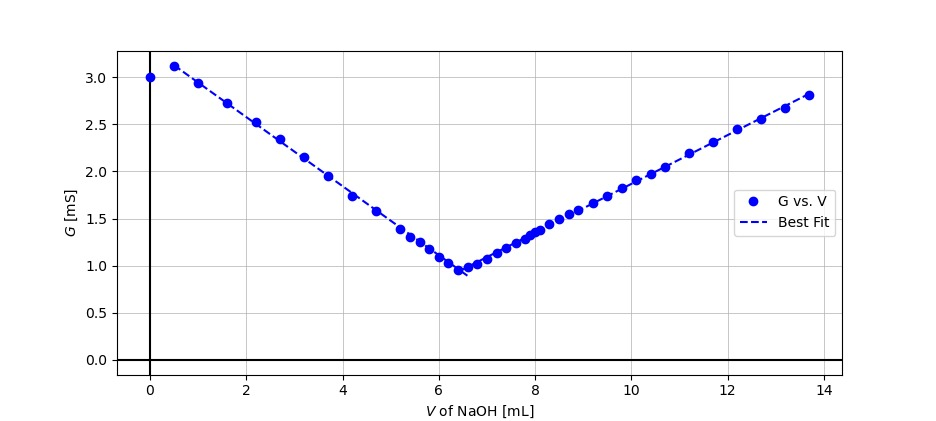
\includegraphics[scale=0.45]{plot.jpeg}
    \caption{Conductance vs. Total vol. of NaOH: Fitting dataset using linear regression}
\end{figure}



\section{Results}

Analyzing the intersection point of the fitted lines, we get the volume of NaOH solution at the endpoint of this conductometric titration = 6.447 mL. Now, \begin{align*}
    N_{\text{NaOH}}V_{\text{NaOH}} &= N_{\text{HCl}}V_{\text{HCl}} \\ N_{\text{HCl}} &= \frac{0.198 \times 6.4}{25} \, \text{N} \approx 0.0507 \, \text{N}\\ 
\end{align*}

Hence, the concentration of the HCl solution was found to be 0.0507 N by this experiment through conductometric titration. 


\end{document}